\documentclass[letterpaper, 10pt]{article}
\usepackage{microtype}
\usepackage{graphicx}
\usepackage{hyperref}

% Bibliography stuff.
\usepackage[
 backend=bibtex,
 bibencoding=ascii,
 sorting=none,
 url=false,       % Do not show url in reference
 doi=false,       % Do not show doi in reference
 isbn=false,    % Do not show isbn link in reference
 eprint=false,    % Do not show eprint link in reference
 maxcitenames=2,  % After two authors use et al. for inline citations
 maxbibnames=9,     % Include up to 9 names in citation
 % firstinits=true  % References using first name initials only
]{biblatex}
\addbibresource{library.bib}

\title{A Quantitative Comparison of Flow Cytometry and Single-Cell Microscopy for Biophysical Measurement}
\author{Griffin Chure$^1$ and Rob Phillips$^{1, 2, *}$}
\date{$^1$ Division of Biology and Biological Engineering, California Institute of
Technology, Pasadena, CA, United States\\ $^2$ Department of Applied Physics,
California Institute of Technology, Pasadena, CA, United States\\ $^*$
\texttt{phillips@pboc.caltech.edu}}
\begin{document}
\maketitle

\section*{Background}
{\bf Comment on the importance of agreement between methods for the same
quantity. Can reference the famed 30\% number for MscL count via
photobleaching and quantitative Western blots. Can also comment on
the previous disbelief in the lab that the flow cytometer would be as
trustworthy as microscopy.\\}}


Allosteric regulation is found across all domains of life, yet we still lack
simple and predictive theories which directly link the experimentally tuneable
parameters of a system to its input-output response. In our recent work,
``Tuning transcriptional regulation through signaling: A predictive theory of
allosteric induction" \cite{RazoMejia2017}, we put forward a general theory of
allosteric transcriptional regulation using the Monod-Wyman-Changeux (MWC)
model and tested its application to one of the most ubiquitous regulatory
architectures in bacteria the simple repression motif \cite{Rydenfelt2014}. In
this regulatory architecture, depicted in Fig. 1(A), expression of a target
gene (in this work, YFP) is under the regulation of a  single transcriptional
repressor which binds to the DNA at a specific binding site (the operator) and
occludes binding of RNA Polymerase (RNAP) to the promoter. However binding of
an inducer can stabilize the inactive state of the repressor, allowing RNAP to
bind the promoter and transcription to occur. Using concepts from statistical
physics and the MWC model of allostery, we can predict the mean fold-change in
gene expression which is defined as the level of expression when repressor
molecules are present in the cell relative to constitutive expression when the
repressor is absent, as is shown schematically in Fig 1(B).

\begin{figure}
  \centering{
  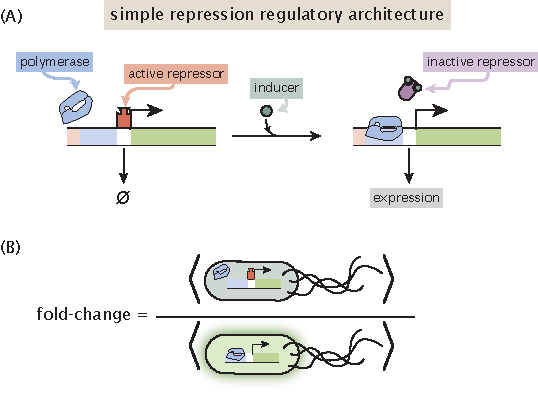
\includegraphics{../figs/fig1}
  \caption{\textbf{The simple repression regulatory architecture.} (A) A
  repressor binds a specific operator site (white rectangle) on the DNA,
  occluding the binding of a polymerase to the promoter (blue rectangle). In
  the presence of an inducer, the inactive state of the repressor is
  stabilized, allowing the polymerase to bind to the promoter and initiate
  transcription. (B) The fold-change in gene expression is defined as the
  expression of a fluorescent protein in a cell containing a given number of
  repressors relative to the constitutively expressing strain with zero
  repressors.}}\label{fig:simple_repression}
\end{figure}



While we invite the reader to see our work for a more detailed derivation, we
simply state here that our expression for the fold-change in gene expression is

\begin{equation}
\mathrm{fold-change} = \left(1 + p_\mathrm{act}(c) {R \over
N_{NS}}e^{-\Delta\varepsilon_{RA}/ k_BT}\right)^{-1}
\label{eq:fold-change}
\end{equation}
where $p_\mathrm{act}$ is the probability of a repressor being active at an
inducer concentration $c$, $R$ is the average number of repressors per cell,
$N_{NS}$ is the number of non-specific binding sites for the repressor,
$\Delta\varepsilon_{RA}$ is the binding energy of the repressor to the DNA,
$k_B$ is the Boltzmann constant and $T$ is the temperature of the system.

Given the MWC definition of allostery, we can write an expression
for $p_\mathrm{act}$ as

\begin{equation}
  p_\mathrm{act} = {\left(1 + {c \over K_A}\right)^n \over \left(1 + {c \over
  K_A}\right)^n + e^{-\Delta\varepsilon_{AI} / k_BT}\left(1 + {c \over
  K_I}\right)^n},
\label{eq:p_act}
\end{equation}

where $K_A$ and $K_I$ are the dissociation constants of the inducer to the
active and inactive repressor, $n$ is the number of allosteric
inducer binding sites on the repressor, and $\Delta\varepsilon_{AI}$ is the
energetic difference between the active and inactive state of the repressor. If
$K_A > K_I$, the inducer binds more tightly to the inactive state of the
repressor than the active state, leading to an increase of gene expression.
Conversely, if $K_A < K_I$, the active state is energetically preferred and the
level of gene expression is lower. The key point of Eq \ref{eq:p_act} is that
the activity of the repressor can be modulated simply by changing the
concentration of the inducer within the cell. In the case of the classic
and well-studied lacI repressor of \textit{Escherichia coli}, addition of the inducer molecule
Isopropylthiogalactopyranoside (IPTG) stabilizes the inactive state of the
repressor and increases gene expression.

We built upon a suite of work which
quantified the copy number $R$ of the LacI repressor and inferred the DNA binding energies
$\Delta\varepsilon_{RA}$ of the three natural operators of the \textit{lac}
operon (colloquially known as O1, O2, and O3), and the allosteric energy
difference $\Delta\varepsilon_{AI}$ \cite{Garcia2011, Brewster2014}. With the data and parameter estimates from
these works, we were left with two unknown quantities, the inducer dissociation
constants $K_A$ and $K_I$. To properly test our theoretical predictions, we sought
to estimate the values of $K_A$ and $K_I$ from single repressor copy number and operator and
then predict the fold-change of other strains. We aimed to test combinations of
six repressor copy numbers, three different operators, all of which over twelve
IPTG concentrations. With each experiment needing and
autofluorescence and constitutive expression control, and the need to perform
between eight and ten biological replicates, the combinatorics revealed that we
needed to perform approximately 3,000 measurements. While this would be a
painstaking exercise for single-cell microscopy, we found that the
high-throughput and automated nature of flow cytometry brought this lofty goal
within reach.

However, we wanted to ensure that the results we would extract from flow
cytometry would agree with those measured through microscopy -- a method we
have used extensively and trusted. To perform this comparison, we measured a
subset of our bacterial strains using both methods, as is diagrammed in Fig 2.
Once the measurements were made, we estimated the most-likely values of the
two dissociation constants and compared their values and errors.


\begin{figure}
\centering{
  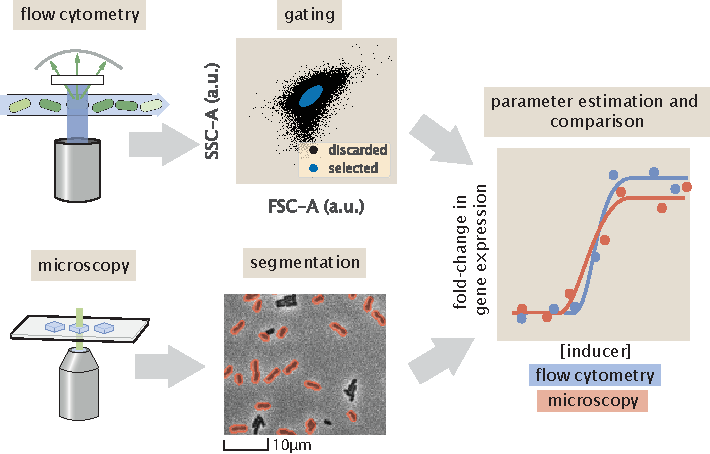
\includegraphics{../figs/fig2}
\caption{\textbf{Experimental flow chart for direct comparison of flow
cytometry and microscopy.} A set of bacterial strains were measured using flow
cytometry and single-cell microscopy. Each method requires a set of automated
processing steps such as gating and image segmentation to generate reproducible
data for parameter estimation.} }\label{fig:flowchart}
\end{figure}

\section*{Results}
Strains with a known repressor copy number $R=260$ with two different operators
(O1 and O2) were measured across all twelve IPTG concentrations along with an
autofluorescence and constitutive expression control. The resulting experimental
measurement is indistinguishable by eye between the two methods. Using these
fold-change measurements, we estimated the most-likely values of the dissociation constants
$K_A$ and $K_I$ using Bayesian inferential methods and can be found in Table 1.
The parameter value estimates are remarkably similar between the two methods. This
is particularly noticing in the overlap between the marginal probability distributions
see in Fig 3(A) and (B). This result shows that the measurement of the fold-change
in gene expression between these two methods are quantitatively indistinguishable.

\begin{table}
  \centering{
  \caption{\textbf{Most-likely parameter value estimates for the dissociation
constants using flow cytometry and microscopy.} The estimation was performed
using Markov chain Monte Carlo as described in Materials \& Methods. The
most-likely value was determined to be the mode of the parameter value
probability distribution and the super- and subscripts correspond to the upper
and lower bounds of the 95\% credible regions.} }
\begin{tabular}{lcr}
  \textbf{Method} & \textbf{Parameter} & \textbf{Value ($\mu$M)}\\
  \hline\\
  Microscopy & $K_A$ & $141^{+42}_{-33}$\\
   & $K_I$ & $0.5^{+0.1}_{-0.1}$\\
  \hline \\
  Flow Cytometry & $K_A$ & $133^{+22}_{-18}$\\
  & $K_I$ & $0.54^{+0.05}_{-0.04}$\\
  \hline
\end{tabular}
\end{table}

\begin{figure}
  \centering{
  \includegraphics{../figs/fig3}
  \caption{\textbf{Estimation of the inducer binding constants between methods.}
  (A) The fold-change in gene expression for two different operators O1 and O2
  with different DNA binding energies. (B) Marginal posterior probability
  distributions for the parameters $K_A$ (top) and $K_I$ bottom obtained from
  the either the microscopy or flow cytometry obtianed data shown in (A).}}
  \label{fig:parameter_estimation}
\end{figure}

While we were interested in the mean expression level of the population for our
experiments, we also examined how similar the intensity distributions between
teh two methods. The expression distributions for a representative experiment
can be seen in Figure 4 (A) and (B) using flow cytometry and microscopy,
respectively. While the measured expression values are not directly comparable
between the two methods, we note that the separation between the expression
distributions as the concentration of IPTG is increased in the sample is distinctly
different. The distributions measured via single-cell microscopy show a significant
separation between adjacent concentrations of IPTG whereas the same distributions
measured through flow cytometry shows significantly higher overlap between
consecutive concentrations of IPTG.

\begin{figure}[ht]
  \centering{
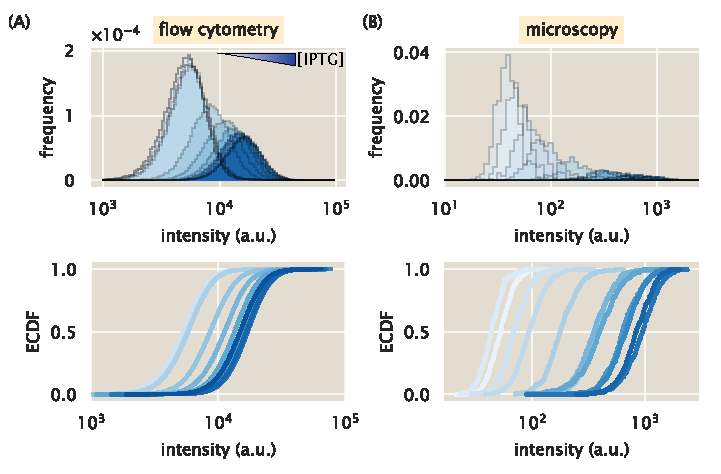
\includegraphics{../figs/fig4}
  \caption{\textbf{Intensity distributions from flow cytometry and microscopy.}
  Histograms (top) and cumulative distributions (bottom) of the expression of a
  strain incubated with IPTG ranging from 0 mM (light blue) to 5 mM IPTG.
  (A) Samples  measured using flow cytometry. (B) Samples measured using
  single-cell microscopy. }}\label{fig:iptg_distributions}
\end{figure}

To quantify the difference between the distributions, we examined a set of
expression measurements from one of our strains maximally induced with 5 mM IPTG,
which is the noisiest distribution. To allow for direct comparison, each distribution
was rescaled between an arbitrary scale of $0$ to $1$ and was then translated
such that the mean of each distribution was zero (Fig. 5(A)). We performed this
procedure for 10 biological replicates using flow cytometry and three for
microscopy. With directly comparable distributions, we numerically computed
variance, skewness, and kurtosis of each distribution Fig. 5(B)). We see that
there is a stark disagreement between the two methods with the distributions
obtained from flow cytometry consistently smaller than those from microscopy.

\begin{figure}
  \centering{
  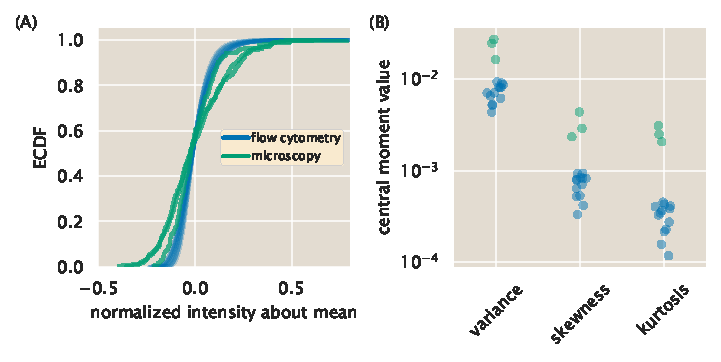
\includegraphics{../figs/fig5}
  \caption{\textbf{Comparison of central moments of the intensity
  distributions.}(A) Expression intensity cumulative distributions for a
  maximally induced strain (5mM IPTG) measured via microscopy (green) and
  flow cytometry (blue). Each distribution was rescaled between 0 and 1.0
  and then recentered with the mean at zero. (B) The central moments normalized for sample
  number were numerically computed for each distribution seen in (A).}
  }\label{fig:central_moments}
\end{figure}

\section*{Discussion}
\textbf{Reiterate the importance of agreement between different methodologies and the
nature of ``knowing". }

In this work, we've shown that for measuring the mean of a distribution, there is no
significant difference between using single-cell microscopy and flow cytometry.
However, if you are interested in the higher moments of the distribution (such
as variance, skewness, and kurtosis), there is a disagreement between the two
methods. As microscopy allows for a larger signal-to-noise ratio of the
measurement, it is likely a better measure of the "true" value for these higher
moments. However, this method is much lower-throughput and requires more manual
intervention for operating the instrument as well as doing the image processing
and proper quantification. While flow cytometry is less sensitive to these
measures of the distributions, the impressively high-throughput nature of the
method makes it particularly attractive, especially if you are interested in
knowing only the mean of the population.


\section*{Materials \& Methods}

All code and data used to make the figures in this application note is stored
in a \href{http://www.github.com/rpgroup-pboc/physical_flow_cytometry}{repository on GitHub}.

\subsection*{Flow Cytometry}
All flow cytometry data was collected on a Miltenyi-Biotec MACSQuant Analyzer
10  flow cytometer generously provided by the Pamela Bj\"{o}rkman lab at
Caltech. All  YFP fluorescence measurements were collected via 488 nm laser
excitation coupled with a 525/50 nm emission filter. All measurements were
taken over the course of two to three hours using automated sampling from a
96-well plate kept at approximately 4$^\circ$ - 10$^\circ$ C on a MACS Chill
96 Rac (Cat. No. 130-094-459). Cells were diluted to a final concentration of
approximately 4 $\times$ 10$^4$ cells per $\mu$L which corresponded to a flow
rate of 2,000 - 6,000 events per second. Acquisition for each well has halted
after 100,000 events were detected.

Flow cytometry data will frequently include a number of spurious events or other
undesireable data points such as cell doublets and debris. To restrict our
analysis to single-cell measurements, we implemented and automated gating
procedure which required no manual selection of desired data. We assume that
the scattering level of the population should be log-normally distributed about
some mean value. We fit a bivariate Gaussian distribution to the log(FSC) vs.
log(SSC) space and restricted the population  to the smallest two-dimensional
region in which 40\% of the data was found.

\subsection*{Single Cell Microscopy}

During the last hour of cell growth, an agarose mounting substrate was prepared
containing the appropriate concentration of the IPTG inducer. This mounting
substrate was composed of M9 minimal medium supplemented with 0.5\% glucose and
2\% agarose (Life Technologies UltraPure Agarose, Cat. No. 16500100). This
solution was heated in a microwave until molten followed by addition of the
IPTG to the appropriate final concentration. This solution was then thoroughly
mixed and a 500 μL aliquot was sandwiched between two glass coverslips and was
allowed to solidify. Once solid, the agarose substrates were cut into
approximately 10 mm × 10 mm squares. An aliquot of one to two microliters of
the diluted cell suspension was then added to each pad. For each concentration
of inducer, a sample of the autofluorescent control, the $\Delta$lacI
constitutive expression control, and the experimental strain was prepared
yielding a total of thirty-six agarose mounts per experiment. These samples
were then mounted onto two glass-bottom dishes (Ted Pella Wilco Dish, Cat. No.
14027-20) and sealed with parafilm.

All imaging was performed on a Nikon Ti-Eclipse inverted fluorescent microscope
outfitted with a custom built laser illumination system and operated by the
open-source $\mu$-Manager control software \cite{Edelstein2014}. The YFP
fluorescence was imaged using a CrystaLaser 514 nm excitation laser coupled
with a laser-optimized (Semrock Cat. No. LF514-C-000) emission filter. For each
sample, between fifteen and twenty positions were imaged allowing for
measurement of several hundred cells. At each position, a phase contrast image,
an mCherry image, and a YFP image were collected in that order with exposures
on a time scale of ten to twenty milliseconds. For each channel, the same
exposure time was used across all samples in a given experiment. All images
were collected and stored in \texttt{ome.tiff} format.

Individual cells and cell clusters were segmented using a constitutively
expressed cytosolic fluorescent marker. Clusters of cells or excessively large
and small cells were restricted from the data set by selecting only those cells
with a projected two-dimensional area of 0.5 $\mu$m$^2$ - 6 $\mu$m$^2$. This set
was further refined by keeping only those cells whose measured eccentricty was
greater than 0.8, ensuring that all measured cells were elliptical in shape.
Once segmented, the mean pixel intensity of the YFP channel for each cell was
measured.

\subsection*{Bayesian Parameter Estimation}
To quantitatively test agreement between flow cytometry and microscopy, we
used Bayesian methods to estimate the most-likely parameter values for the
binding constants $K_A$ and $K_I$ of the inducer IPTG to the active and
inactive repressor, respectively. We computed the probability distribution of
the value of each parameter geven the data $D$ which by Bayes' theorem is given
by

\begin{equation}
  P(K_A, K_I \, \vert \, D) \propto P(D\, \vert \, K_A, K_I)P(K_A, K_I)
  \label{eq:bayes_thm}
\end{equation}
where $D$ is all of the data composed of independent variables (such as repressor
copy number $R$, inducer concentration $c$, and repressor-DNA binding energy $\Delta\varepsilon_{RA}$).
The quantity $P(D\, \vert \, K_A, K_I)$ is the likelihood of observing the
data given the parameter values for the dissociation constants. Our
prior knowledge of the dissociation constant values without considering the data $D$
are described by $P(K_A, K_I)$.

We assume that the $n$, individual measurements of fold-change are independent and
Gaussian distributed about a mean value dictated by Eq. \ref{eq:fold-change}
and a variance $\sigma$,

\begin{equation}
  P(D\, \vert \, K_A, K_I) = \prod\limits_i^n\mathrm{Normal}\left(\mu = \mathrm{fold-change}\left(K_A, K_I, D^{(i)}\right),
  \sigma\right).
  \label{eq:likelihood}
\end{equation}

For our prior distribution $P(K_A, K_I)$, we can be maximally uninformative and
assume that the parameter value can be any value within a given range. Broth
mathematically and numerically, it is convenient to define $\tilde{k}_A = -log{K_A \over 1\,\text{M}}$
and $\tilde{k}_I = -log{K_I \over 1\,\text{M}}$ and fit these parameters on a
log scale. As dissociation constants are scale invariant, meaning that a change
from 10 $\mu$M to 1 $\mu$M leads to an equivalent increase in affinity as a
change from 1 $\mu$M 0.1 $\mu$M.  With these definitions in place, we can
write our prior distribution as

\begin{equation}
P(K_A, K_I) = {1 \over \left(\tilde{k}_A^\text{max} - \tilde{k}_A^\text{min}\right)}{1 \over \left(\tilde{k}_I^\text{max} - \tilde{k}_I^\text{min}\right)}
\end{equation}
In this analysis, we  defined the $\tilde{k}_A$ and $\tilde{k}_I$ ranges uniform
on the range -7 to 7, although we note that this particular choice does not affect
the outcome provided the range is sufficiently wide.

We also must include any prior knowledge about the sample variance $\sigma$ defined
in Eq \ref{eq:likelihood}. As is typically used, we chose a Jeffreys prior \cite{Sivia2006}
for $\sigma$ yielding,

\begin{equation}
  P(\sigma) = {1 \over \sigma}.
  \label{eq:Jeffreys}
\end{equation}

To perform the estimation, we used Markov Chain Monte Carlo to sample from the
posterior probability distribution $P(\tilde{k}_A, \tilde{k}_I, \sigma\,\vert\, D)$,
and computed the marginal distributions for $K_A$ and $K_I$.


\printbibliography
\end{document}
